\chapter{\label{intro}Introduction}
Experimental high-energy physics (HEP) is focused on two basic goals that are interconnected. It seeks for novel particles associated with physics beyond the Standard Model(SM) with increasing precision and probes for the Standard Model(SM) with increasing precision. The standard model had correctly predicted the existence of $W^\pm$ and Z bosons along with the top quark\cite{Salam:1964ry}\cite{GLASHOW1961579}\cite{PhysRevLett.19.1264}\cite{10.1143/PTP.49.634}. The discovery of the Higgs boson in 2012 at the LHC (CERN) further uphold the model\cite{Aad_2015}.

The \autoref{fig:my_figure_1} shows the known three generations of matter for leptons and quarks, along with the gauge bosons and one Higgs boson. The leptons and quarks make up matter, whereas the gauge bosons mediate the interactions among them. All massive fundamental particles in the Standard Model get their masses through the Brout-Englert-Higgs (BEH) mechanism.\cite{PhysRevLett.13.321}\cite{Higgs:1964pj}

For both SM and BSM, rare signals need to identify from vast backgrounds. This becomes an important issue as the amount of pile-up collisions with additional protons in the bundle at  HL-LHC increases significantly\cite{https://doi.org/10.48550/arxiv.1807.02876}. This have been helped by the introduction of machine learning techniques. Machine learning algorithms are already state-of-the-art in event and particle identification, energy estimation, and pile-up suppression applications in HEP. By using machine learning techniques to study the laws governing the structure of matter and  its interactions. High energy physics seeks to discover the basic properties of the physical universe.\cite{Baldi2014}.\\
Observing these particles and measuring their properties can provide important insights into the properties of the matter\cite{Higgs_snowmass}. Such discoveries require powerful statistical methods, 
and machine learning tools to play a critical role. Given the limited quantity and expensive data, improvements in analytical tools directly boost particle discovery potential. 



% Chapter 1: Introduction
%     \begin{itemize}
%         \item SM
%         \item BSM
%         \item VLQ
%         \item Signal and Background Topology 
%         \item CMS
%         \item Objective of your experiment
%             \end{itemize}
    
% chapter 2: Machine Learning
% Chapter 3:  Simulated Samples
% \begin{itemize}
%     \item About CMS
%     \item about how can it be helpful for your work
%     \item how data are simualtad 
%     \item how you obtained the data
%     \item as written in the last report

% \end{itemize}

% Chapter 4:Analysis Strategies\\

% chapter 5:- Results and Discussion\\
% ch-6: summary and Conclusion



\section{Standard Model and shortcomings}

The Standard Model of particle physics(\autoref{fig:my_figure_1})is a model attempt to explain  events and phenomena in the universe. The Standard Model(SM) of Fundamental Interaction, which has  been successfully tested for the past 30 years, validates its dynamics in both  the gauge sector and  flavor structure, including a compelling confirmation of the cause of the observed parity violations(P) and combined charge and parity symmetry (CP). However, this is an incomplete theory and does not explain many  observed or unobserved events, such as:
\begin{figure}[H]
    \centering
    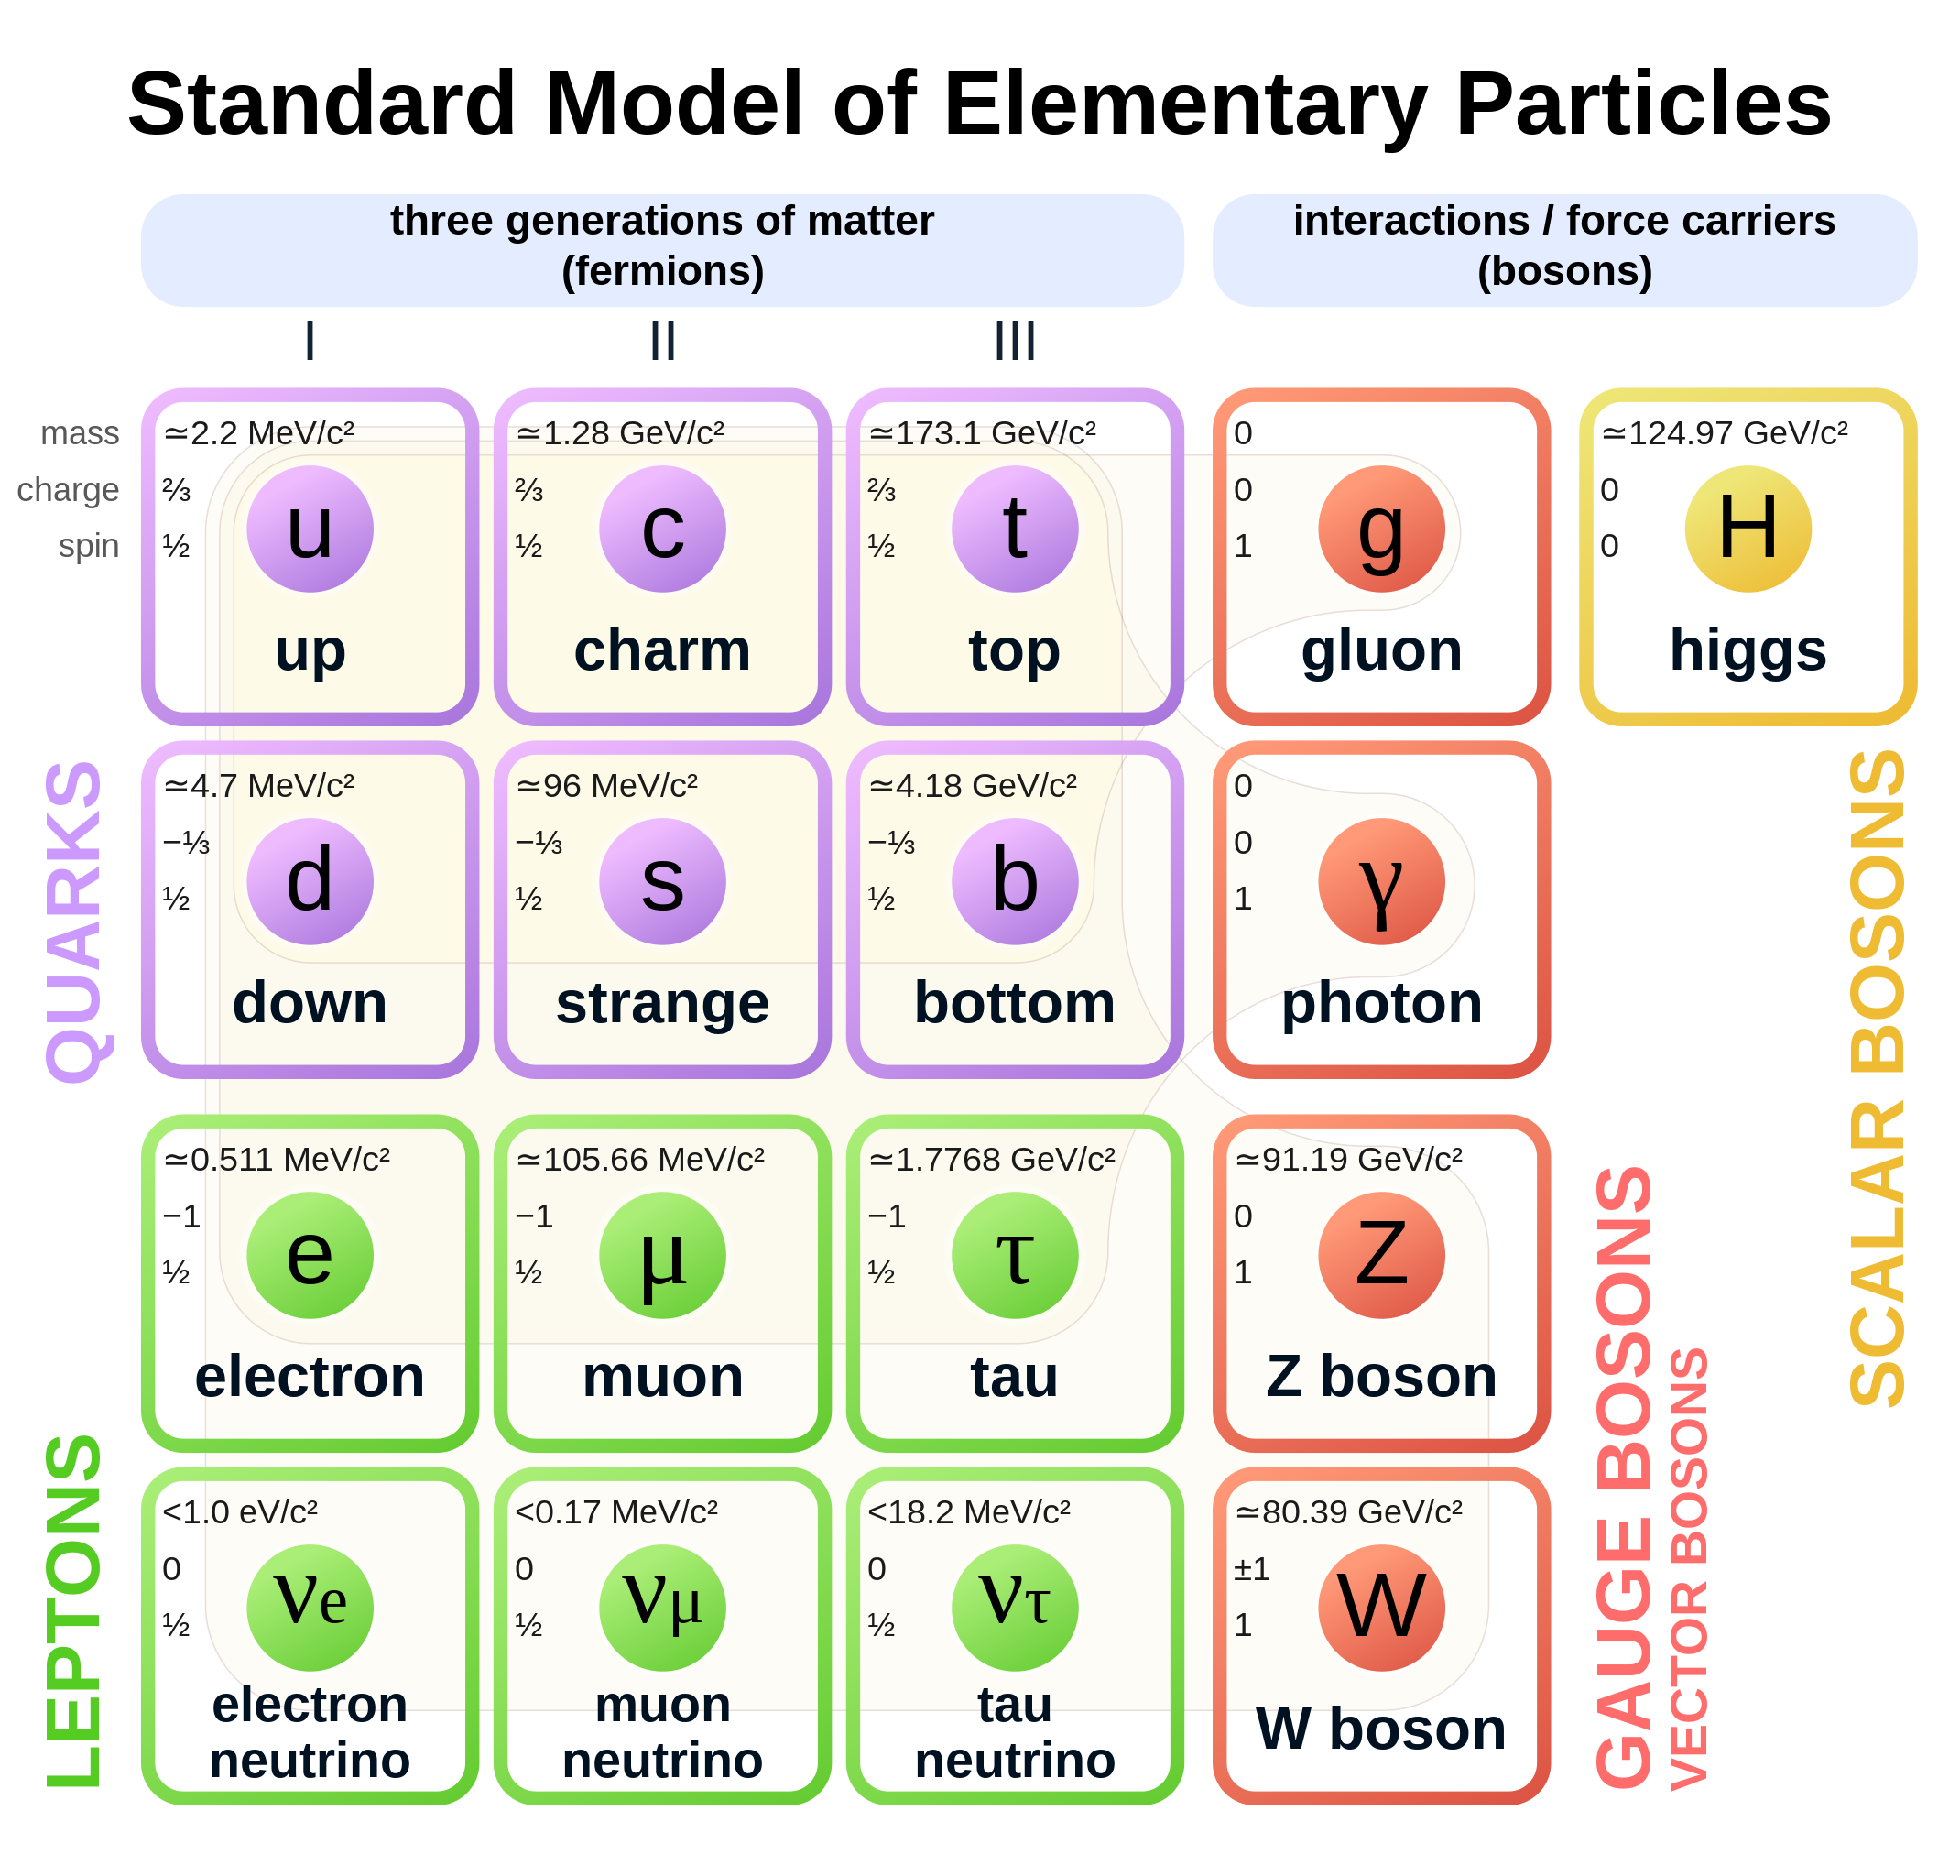
\includegraphics[scale =0.1]{figure_1/Standard_Model_of_Elementary_Particles.svg.png}
    \caption{Standard Model of particle physics[1]}
    \label{fig:my_figure_1}
\end{figure}
\begin{itemize}
    \item The model does not explain \textbf{gravity}, but it does explain to some extent the physical confirmation of  theoretical particles known as gravitons. Although it corresponds to  strong interaction and electroweak interaction, the Standard Model does not consistently explain the canonical theory of gravity and the general theory of relativity from the viewpoint of quantum field theory. One reason for this is that quantum field theory in the field of gravity usually collapses before reaching the Planck scale. As a result, we do not have a reliable theory of the very early universe.
    
    \item \textbf{Hierarchy problem:-} The Standard Model introduces particle mass through a process known as spontaneous symmetry breaking caused by the Higgs field. In the Standard Model, the Higgs mass undergoes some very large quantum corrections due to the presence of virtual particles (mainly virtual top quarks). These corrections are much larger than the true mass of the Higgs. This means that the Higgs bare mass parameters of the Standard Model need to be fine-tuned so that the quantum correction is almost completely canceled\cite{Aad_2015}. This level of tweaking is considered unnatural by many theorists.
 \item \textbf{Neutrino Oscillation:-} According to the Standard Model, neutrinos are massless particles. However, neutrino oscillation experiments have shown that neutrinos  have mass. The neutrino mass term can be manually added to the Standard Model, which poses a new theoretical problem\cite{neutino_1}. For example, the mass term must be very small, and it is not clear whether the mass of neutrinos is generated in the same way as the mass of other elementary particles  in the Standard Model.\cite{Ellis_2020}
 \item \textbf{Matter anti-Matter asymmetry:-} The universe is mainly composed of  matter. However, the Standard Model predicts that if the initial conditions of the universe do not contain an imbalanced amount of matter compared to antimatter, matter and antimatter should be formed in (almost) equal amounts\cite{Dasgupta_2020}. However, the Standard Model does not have a mechanism to properly explain this asymmetry.
 \item \textbf{Quantum triviality:-} It suggests that it may not be possible to build a consistent quantum field theory using basic scalar Higgs bosons. This is sometimes referred to as the Landau pole problem.
 \item \textbf{Strong CP problem:-} Theoretically, it can be argued that the Standard Model should contain terms that break CP symmetry (matter to antimatter) in the area of strong interaction. However, no such violation was found experimentally. This means that the coefficients in this term are very close to zero.
\item Unable to explain the baryon asymmetry
\item unable to describe the general relativity and universe's accelerating expansions
\end{itemize}   

The another theory, the Beyond Standard Model(BSM) had to deal with the basic parameters of the Standard Model, the strong CP problem, neutrino oscillations, matter-to-matter asymmetry, and the inability to explain the nature of dark matter and dark energy \cite{https://doi.org/10.48550/arxiv.1202.1391}. Many theories have been developed to extend  SM to address some of the above issues. Some of these models are supersymmetry (SUSY)\cite{MARTIN_1998}, right-handed neutrino seesaw models \cite{neutrino_mass_model}, vector-like quarks and extra-dimensional prediction models. Vector like Quark (VLQ) model predicts the presence of giant particles  Non-chiral quark. These quarks can be formed by proton-proton (pp) collisions at 13 TeV at the LHC. VLQ is the subject of this research and will be discussed in detail in the next section.



%  Surprisingly, all these extensions of  SM predict new particles. The SUSY model predicts the presence of  supersymmetric partners for all SM particles with different spin  units. This means that all fermions have supersymmetric boson partners and vice versa. 
%  The seesaw model introduces a sterile heavy right-handed neutrino to explain this much. 
%  A small left-handed neutrino mass that appears in  SM. The additional dimensions predict the existence of some new dimensions in addition to the usual four space-time dimensions. These may explain why gravity is so much weaker than  other fundamental forces of nature. According to these theories, gravitons (carriers of gravitational force) can penetrate these additional dimensions, but other SM particles cannot. Vectorlike Quark (VLQ) model predicts the presence of giant particles  Non-chiral quark. These quarks can be formed by proton-proton (pp) collisions at 13 TeV at the LHC. VLQ is the subject of this research and will be discussed in detail in the next section.

\section{Vector-like Quarks(VLQ)}


SM has only chiral fermions. That is, the left-handed and right-handed fermionic fields are converted. 
 It is different for SU(2) gauge conversion. As a result, the Dirac mass term m becomes $\psi\Bar{\psi} $. 
 In this theory, it is  forbidden  to maintain the gauge invariance of SU (2) Lagrangian\cite{Aguilar_Arevalo_2018}. Therefore, SM will be charged  Fermions gain mass via the (BroutEnglertHiggs) BEH mechanism\cite{PhysRevLett.13.321}\cite{Higgs:1964pj}. In particular,  W bosons only interact with SM left-handed fermions. \\
 However, some theoretical models predict the existence of new heavy quarks that are not Chiral nature. Such models include compound Higgs, Randall Sundrum models\cite{Randall_1999}, and Grand. 
 Unified Theory (GUT)\cite{Kang_2008} and Little Higgs model\cite{Arkani_Hamed_2002}. Unlike SM quarks, these are quarks 
 Vector coupled to the charged current. These quarks are heavier partners for top and bottom quarks. That is, a T quark with a charge of $ \frac{2}{3} $ e and a B quark with a charge of $ \frac{1}{3} $ e. Or some models predict that T-quarks can solve hierarchical problems. 
 They help cancel the divergent quantum loop correction introduced by the top quark 
 To the Higgs mass. These new quarks can interact with  SM particles and  decay to one-third. 
 Generation quarks and  heavy bosons. For such non-chiral fermions, the Dirac mass term m $ \psi\Bar{\psi} $ is not prohibited. The only way to determine the mass of these particles is to find them experimentally.  Previous searches for these VLQs were performed by both ATLAS and CMS at $ \sqrt {s} $ = 7, 8, and 13TeV \cite{Aad_2014}. It is a colored spin 1/2 fermion \cite{VLQ_1}. 
 Your left-handed and right-handed com 
 Components are transformed in the standard model gauge group as well. Therefore different 
 SM chiral quarks, their masses are not produced by the Yukawa interaction with the Higgs. 
 It is a  boson and has little effect on the cross-section of the Higgs boson. Various modifications 
%  The new physics els introduces vector-like quarks. 
%  Such models include composite Higgs models \cite{neutrino_mass_model}, Little-Higgs model \cite{Perelstein_2004} \cite{Matsedonskyi_2013},  Extradimension model [\cite{Randall_1999}, etc. 
 This paper investigates the specific separation of the Tprime ($ T^`$) quark decay topology  described in the next section.
 
 
 







The vector-like top quark partner $T^`$ has two generation modes. One is due to pair production  
 There is a strong interaction and the other is a single production mode with electroweak interactions. The $T^'$ quark is combined with bW, tZ, or tH into the corresponding $ T^'$ quark. 
 It will collapse. In this paper, this study is a single top quark partner $T^'$ like a vector generated in a proton-proton (pp) collision at $ \sqrt{s} $ = 13TeV, pp $\longrightarrow$ $T^'$. The focus is on electroweak generation. $T^'$ qb is a channel from the Higgs boson to two photons (H $\longrightarrow\gamma\gamma$) and is generated by the Higgs boson decay $T^`$ $\longrightarrow$ tH. The reading order (LO) Feynman diagram is shown in \autoref{fig:my_label_Feynman}. This search is designed to be sensitive to  top quark lepton decay and Higgs boson decaying into two photons. The experimental features are the resonance peak of the invariant mass spectrum of the two photons and another resonance peak of the invariant tH  mass spectrum. This search is motivated by the excess observed  at $T^'\longrightarrow$ tH (bb) at 13TeV. 
The search for the $T^'$ quark from the large backgrounds processes have been helped with the use Deep neural network which have been discussed briefly in next section.

\begin{figure}[H]
    \centering
    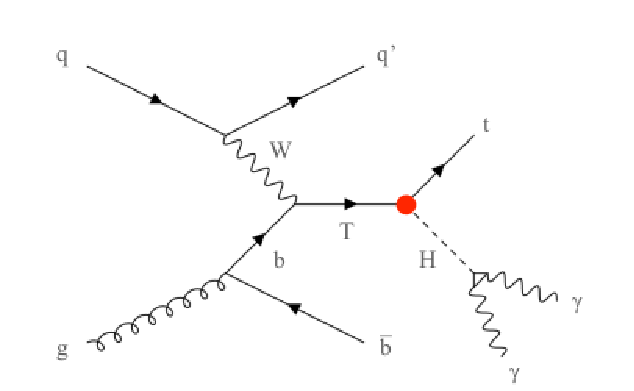
\includegraphics{figure_4/Fynnman.pdf}
    \caption{Feynman diagram of single production for single ${T^'}$ production.}
    \label{fig:my_label_Feynman}
\end{figure}

\section{Deep Neural Network(DNN)}
Neural networks, also known as artificial neural networks(ANN), are structures inspired
by the human brain and also mimic the connectivity of biological signals to one another, as in \autoref{fig:my_label_NN_ANNN}.
Neural networks, apart from being universal approximators (i.e., they approximate probability densities or posterior probabilities to arbitrary accuracy), provide a very practical tool because of the relatively small computational times required in their training ( in a majority of applications in HEP). The fast convergence as well as the robustness in supervised learning of multilayer perceptrons are due to efficient and powerful algorithms developed in recent years.

The neurons and synapses have been replaced with connected layers of nodes ( neurons)
and edges. The node takes the input as a real number (the weighted sum of the connected outputs from the previous layer) and performs a non-linear transformation to form that output\cite{Bourilkov_2019}.
These non-linear transformation functions are known as the activation function. A typical activation function is: Sigmoid (logistics) and Tanh (output is limited to the following for all input values), and the normalized linear unit ReLU (max (0, x) or the positive part of the argument. Each neural network consists of at least an input, an output, and one or more hidden layers. This is part of Deep learning. We represent deep NN as DNN. The learning can be supervised depending on pairs of inputs with known outputs for training, or unsupervised,
or semi-supervised. A cost or loss function measures the “distance” between the current
and the desired outcomes, where our main goal is to make a loss as little as possible to
train the model. Traditional optimization aims to minimize the cost function of available (training) data. The main goal of ML is to generalize or minimize the cost of hidden or  test data. At each step,  backpropagation based on the differential chain rule can adjust the weights of all edges to reduce the cost function slightly. This is Stochastic Gradient Descent (SGD), which further in detailed discussed in \autoref{ML}.

\begin{figure}[h]
    \centering
    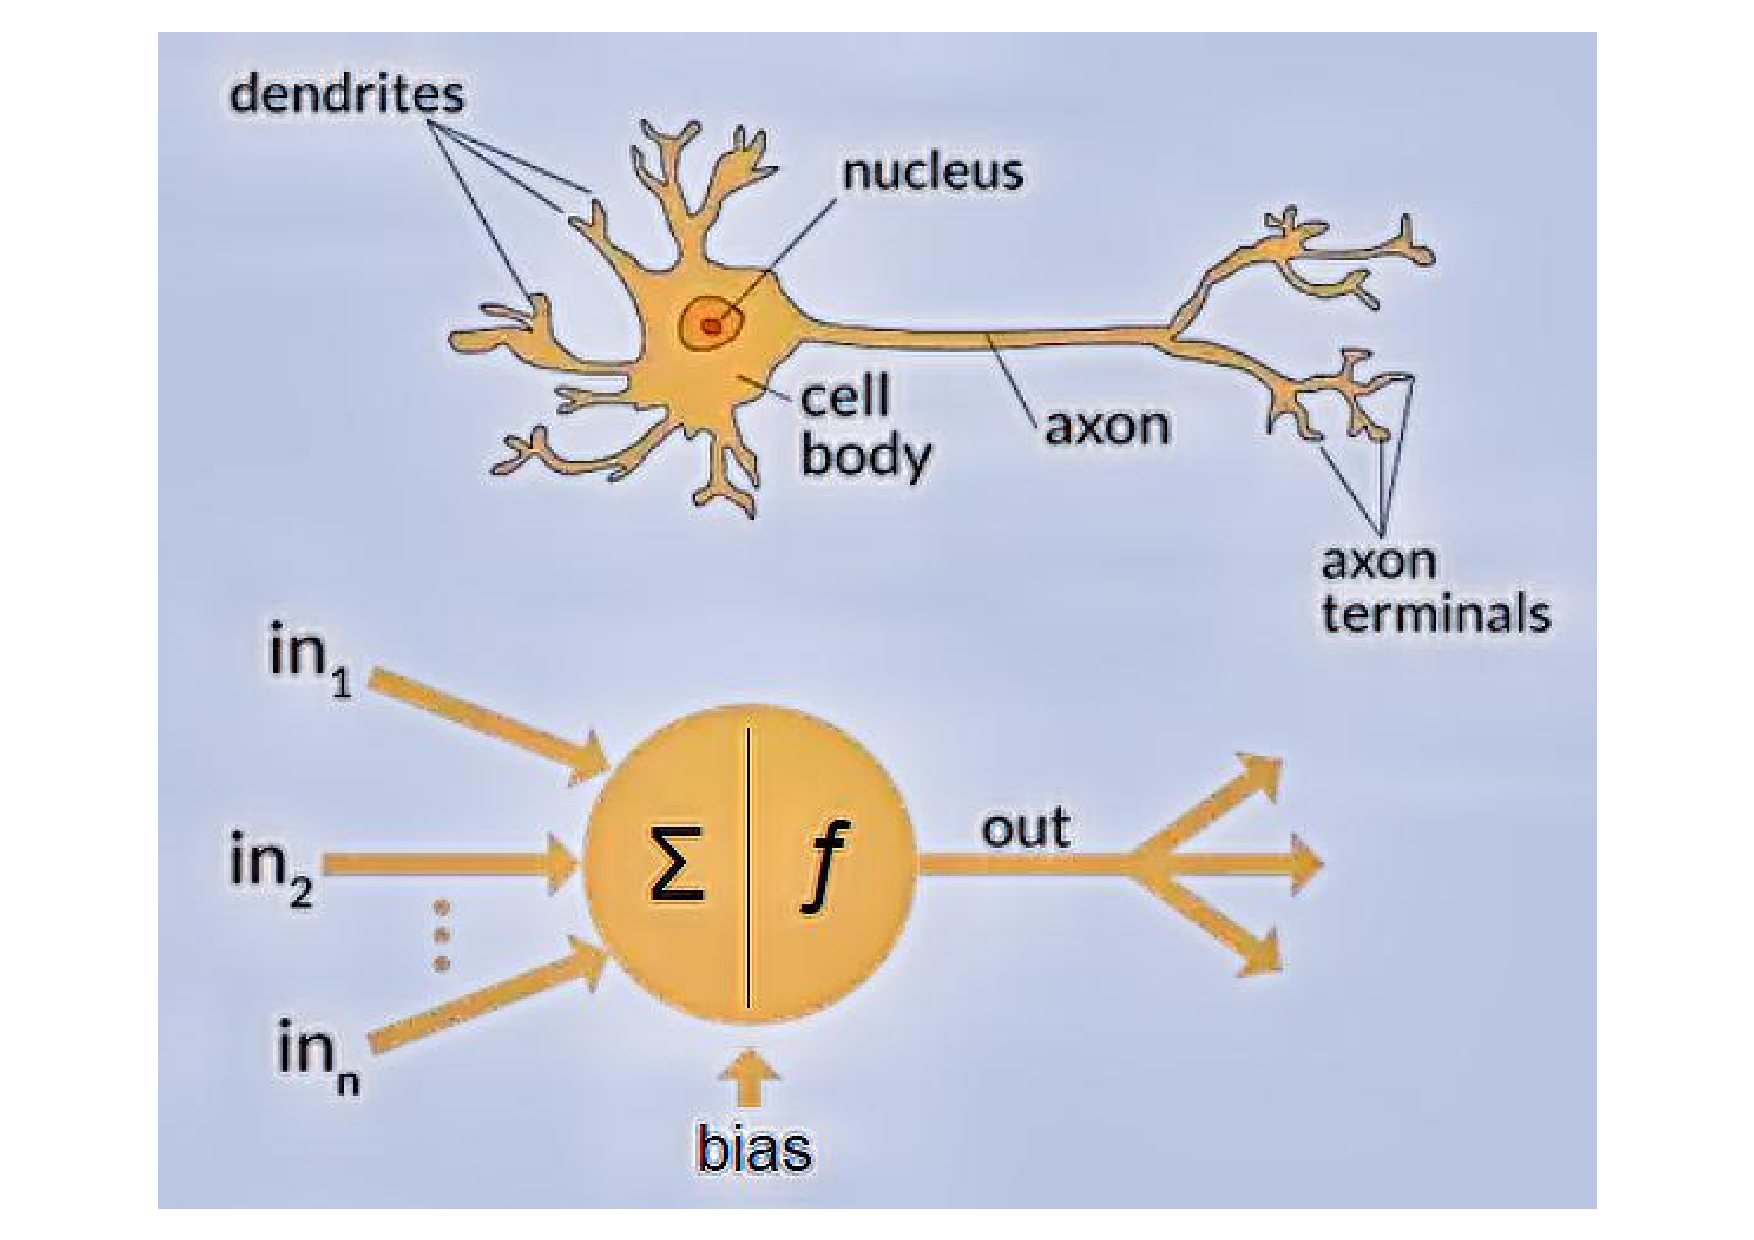
\includegraphics[scale=0.2]{Figure/img_neuron.pdf}
    \caption{A biological and an artificial neuron}
    \label{fig:my_label_NN_ANNN}
\end{figure}

\section{Signal and Background}
The Deep Neural network(DNN) has been trained with the Tprime($T^'$) at different mass point as signal and with standard model higgs(SMH) as the backgrounds which also decays leptonically. The different SMH backgrounds used in training are ttH($\longrightarrow$ $\gamma \gamma$), tH($\longrightarrow$ $\gamma \gamma$)q, VBFH($\longrightarrow$ $\gamma \gamma$), VH($\longrightarrow$ $\gamma \gamma$), and ggH(H($\longrightarrow$ $\gamma \gamma$).

The DNN training output further tested over the Non-Resonant background(tt$\gamma \gamma$, ttJets, tgJets, gJets, and DiphotonJets), which plotted in ratio plot after normalizing with the data and the monte carlo, which have been further discussed in details in \autoref{signal_background}. 


%%%Objective of the experiment%%%%
Further,the analysis strategy with the discussion of the combined tools used for the exclusion limit calculation for the different mass point is discussed in \autoref{AN} and the output results can be seen in the \autoref{R_D}.















    







% \url{https://lhc-machine-outreach.web.cern.ch/lhc_in_pictures.htm}
% \url{https://lhc-closer.es/taking_a_closer_look_at_lhc/1.standard_model}


% \noindent\fbox{%
%     \parbox{\textwidth}{%
% 1.   Dawson, S. et al. Higgs Working Group Report of the
% Snowmass 2013 Community Planning Study, Preprint at
% http://arxiv.org/abs/1310.8361 (2013).
% https://home.cern/science/physics/matter-antimatter-asymmetry-problem
% 2. Neyman, J. & Pearson, E. Philosophical Transactions of
% the Royal Society 231, 694–706 (1933).
% 3.  Womersley, J. (February 2005). "Beyond the Standard Model" (PDF). Symmetry Magazine. Archived from the original (PDF) on 2007-10-17. Retrieved 2010-11-23.
% 4. S. P. Martin, Adv. Ser. Direct. High Energy Phys.21 (2010), 1-153, arXiv:hep-ph/9709356.
% 5 S.F. King, Rept.Prog.Phys. 67 (2004) 107-158, arXiv:hep-ph/0310204
% 6 M. Shifman, Int.J.Mod.Phys.A25:199-225, 2010, arXiv:0907.3074.
% R. Contino, L. Da Rold, and A. Pomarol, “Light custodians in natural composite Higgs
% models”, Physical Review D 75 (March, 2007) 055014,
% doi:10.1103/PhysRevD.75.055014. arXiv: hep-ph/0612048.
% [6] R. Contino, T. Kramer, M. Son, and R. Sundrum, “Warped/Composite Phenomenology
% Simplified”, Journal of High Energy Physics 2007 (May, 2007) 074–074,
% doi:10.1088/1126-6708/2007/05/074. arXiv: hep-ph/0612180.
% [7] D. B. Kaplan, “Flavor at ssc energies: A new mechanism for dynamically generated
% fermion masses”, Nuclear Physics B 365 (November, 1991) 259–278,
% doi:10.1016/S0550-3213(05)80021-5.
% [8] M. J. Dugan, H. Georgi, and D. B. Kaplan, “Anatomy of a composite Higgs model”,
% Nuclear Physics B 254 (January, 1985) 299–326,
% doi:10.1016/0550-3213(85)90221-4.
% [9] S. Blasi and F. Goertz, “Softened Goldstone-Symmetry Breaking”, Physical Review Letters
% 123 (November, 2019) 221801, doi:10.1103/PhysRevLett.123.221801. arXiv:
% 1903.06146.
% [10] M. Perelstein, M. E. Peskin, and A. Pierce, “Top Quarks and Electroweak Symmetry
% Breaking in Little Higgs Models”, Physical Review D 69 (April, 2004) 075002,
% doi:10.1103/PhysRevD.69.075002. arXiv: hep-ph/0310039.
% [11] O. Matsedonskyi, G. Panico, and A. Wulzer, “Light Top Partners for a Light Composite
% Higgs”, Journal of High Energy Physics 2013 (January, 2013) 164,
% doi:10.1007/JHEP01(2013)164. arXiv: 1204.6333.
% [12] M. Schmaltz and D. Tucker-Smith, “Little Higgs Review”, Annual Review of Nuclear and
% Particle Science 55 (December, 2005) 229–270,
% doi:10.1146/annurev.nucl.55.090704.151502. arXiv: hep-ph/0502182.
% [13] L. Randall and R. Sundrum, “A Large Mass Hierarchy from a Small Extra Dimension”,
% Physical Review Letters 83 (October, 1999) 3370–3373,
% doi:10.1103/PhysRevLett.83.3370. arXiv: hep-ph/9905221.
%     }%
% }